\documentclass[11pt, a4paper]{article}

\usepackage{amsmath}
\usepackage{amssymb}
\usepackage{pgfplots}
\usepackage{algorithm}
\usepackage{placeins}
\usepackage{algorithmic}
\usepackage{booktabs}

\begin{document}

\title{THE PERCEPTRON}
\date{}
\maketitle

The perceptron is a learning algorithm for binary classification of real valued vectors. 

\section{Introduction}

The perceptron binary classifier can be thought of as the following function,

\begin{align*}
	f(\boldsymbol{x}) = \left\{                       
	\begin{array}{ll}                                 
	1\ \text{if}\ \boldsymbol{w}^T \boldsymbol{x} > 0 \\
	0\ \text{otherwise}                               \\
	\end{array}                                       
	\right.                                           
\end{align*}

\begin{figure}[htbp]
	\centering
	\begin{tikzpicture}
		\tikzstyle {point line} = [line width=0.15em]
														    
		\draw[-latex] (-3,0) -- (3,0) node[right]{$x_1$};
		\draw[-latex] (0,-2) -- (0,2) node[left]{$x_2$};	
											    
		\draw[dashed] (-1, 2) -- (1, -2);
		\draw (1, -2) node [below right] {Separating Plane};   
										
		\draw[very thick,->, >=stealth] (0, 0) -- (1, 0.5);
		\draw (1, 0.5) node [above right] {$\vec{\boldsymbol{w}}$};  
										
		\draw (-0.1, -0.3) node [below left] {$f(\boldsymbol{x}) < 0$};   
		\draw (0.5, 0) node [below right] {$f(\boldsymbol{x}) > 0$};   				
	\end{tikzpicture}
\end{figure}

One severe limitation of this formulation is that the separating hyperplane always passes through origin which might be undesirable in many cases. However, this limitation can be overcome in the following way,

\begin{align*}
	f(\boldsymbol{x}) = \left\{                           
	\begin{array}{ll}                                     
	1\ \text{if}\ \boldsymbol{w}^T \boldsymbol{x} + b > 0 \\
	0\ \text{otherwise}                                   \\
	\end{array}                                           
	\right.                                               
\end{align*}

The bias term $b$ frees the separating hyperplane from origin. Additionally, we can employ a trick to simplify the expression as follows.

\begin{align*}
	f(\boldsymbol{x}) = \left\{                                                                    
	\begin{array}{ll}                                                                              
	1\ \text{if}\ \begin{pmatrix} \boldsymbol{w}^T, b \end{pmatrix} \begin{pmatrix} \boldsymbol{x} \\ 
	1 \end{pmatrix} > 0                                                                            \\
	0\ \text{otherwise}                                                                            \\
	\end{array}                                                                                    
	\right.                                                                                        
\end{align*}

Hence, by increasing the dimension of input by one and defaulting the intercept on the new dimension to 1 for every input vector, any separating hyperplane in the old dimensional space 
becomes a hyperplane passing through origin in the new dimensional space. This simplifies the mathematics without constraining the classifier.

The vector $\vec{\boldsymbol{w}}$ is learned from training data as usual. The algorithm for learning the same is presented in the next section. 

\section{Learning Algorithm}

The training data consists of $N$ pairs of $d$-dimensional real input vectors $\boldsymbol{x}_i$s and the output binary labels $y_i$s. For mathematical convenience, positive output labels are denoted by $+1$ and negative output labels by {-1}. 
The learning algorithm makes the following assumptions:

\begin{itemize}
	\item It is assumed that the input vectors have already been extended to account for the bias term.
	\item The training data is assumed to be linearly separable at origin. So, there exists a unit vector $\boldsymbol{w}^*$ such that $y_i\boldsymbol{w}^{*T}\boldsymbol{x_i} > \gamma \ \ \forall i \ \ \text{where}\ \ \gamma > 0$.
	\item It is assumed that all training input vectors are finite.
\end{itemize} 

The algorithm is defined as follows.

\begin{algorithm}
	\renewcommand{\thealgorithm}{}
	\caption{The Perceptron Learning Algorithm}
	\begin{algorithmic} 
		\STATE $k \leftarrow 1$
		\STATE $\boldsymbol{w}_k \leftarrow 0$
						
		\WHILE {there exists $j \in \{1, 2, .., N\}$ such that $ y_j\boldsymbol{w}^{*T}\boldsymbol{x_j} <= 0$ }
		\STATE {pick $i \in \{1, 2, .., N\}$ such that $ y_i\boldsymbol{w}^{*T}\boldsymbol{x_i} <= 0$}
		\STATE $\boldsymbol{w}_{k+1} \leftarrow \boldsymbol{w}_k + y_i \boldsymbol{\boldsymbol{x}_i}$
		\STATE $ k \leftarrow k + 1$
		\ENDWHILE
		\RETURN $\boldsymbol{w}_k$
	\end{algorithmic}
\end{algorithm}

\section{Example}

The algorithm is illustrated on a very simple example.

\begin{figure}[htbp]
	\centering
	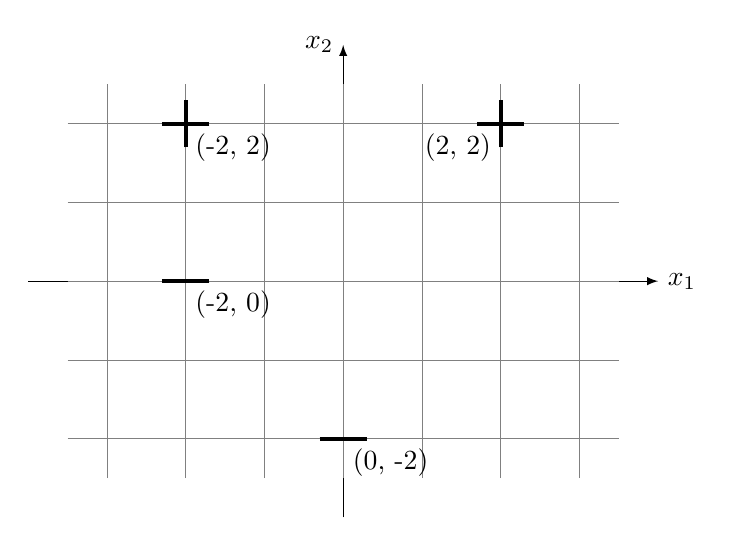
\begin{tikzpicture}
		\tikzstyle {point line} = [line width=0.15em]
								    
		\draw[-latex] (-4,0) -- (4,0) node[right]{$x_1$};
		\draw[-latex] (0,-3) -- (0,3) node[left]{$x_2$};
									
		\draw[help lines] (-3.5,-2.5) grid (3.5,2.5);
									
		\draw[point line] (-1.7,0) -- (-2.3,0);
		\draw[point line] (-0.3,-2) -- (0.3,-2);      
						
		\draw[point line] (-1.7,2) -- (-2.3,2);
		\draw[point line] (-2,1.7) -- (-2,2.3);  
						
		\draw[point line] (1.7,2) -- (2.3,2);
		\draw[point line] (2,1.7) -- (2,2.3); 	
						
		\draw (-2, 2) node [below right] {(-2, 2)};
		\draw (2, 2) node [below left] {(2, 2)};
		\draw (-2, 0) node [below right] {(-2, 0)};
		\draw (0, -2) node [below right] {(0, -2)};
	\end{tikzpicture}
\end{figure}

\FloatBarrier

\subsection{Iteration 1}

\begin{align*}
	\boldsymbol{w}_1 = \begin{pmatrix} 0 \\ 0 \end{pmatrix}
\end{align*}

\begin{table}[htbp]
	\centering
	\begin{tabular}{|c|c|c|}
		\toprule
		$\boldsymbol{x}$    \\
		\midrule
		$\begin{pmatrix} -2 \\ 0 \end{pmatrix}$ & -1 & 0 \\
		$\begin{pmatrix} 0  \\ -2 \end{pmatrix}$ & -1 & 0 \\
		$\begin{pmatrix} -2 \\ 2 \end{pmatrix}$ & 1 & 0 \\
		$\begin{pmatrix} 2  \\ 2 \end{pmatrix}$ & 1 & 0 \\
		\hline
	\end{tabular}
\end{table}

\subsection{Iteration 2}

\begin{align*}
	\boldsymbol{w}_2 & = \begin{pmatrix} 0 \\ 0 \end{pmatrix} + (-1)  \begin{pmatrix} -2 \\ 0 \end{pmatrix}  \\
	                 & = \begin{pmatrix} 2 \\ 0 \end{pmatrix}
\end{align*}

\begin{table}[htbp]
	\centering
	\begin{tabular}{|c|c|c|}
		\toprule
		$\boldsymbol{x}$    \\
		\midrule
		$\begin{pmatrix} -2 \\ 0 \end{pmatrix}$ & -1 & 4 \\
		$\begin{pmatrix} 0  \\ -2 \end{pmatrix}$ & -1 & 0 \\
		$\begin{pmatrix} -2 \\ 2 \end{pmatrix}$ & 1 & -4 \\
		$\begin{pmatrix} 2  \\ 2 \end{pmatrix}$ & 1 & 4 \\
		\hline
	\end{tabular}
\end{table}

\FloatBarrier

\subsection{Iteration 3}

\begin{align*}
	\boldsymbol{w}_3 & = \begin{pmatrix} 2 \\ 0 \end{pmatrix} + (-1)  \begin{pmatrix} 0 \\ -2 \end{pmatrix}  \\
	                 & = \begin{pmatrix} 2 \\ 2 \end{pmatrix}
\end{align*}

\begin{table}[htbp]
	\centering
	\begin{tabular}{|c|c|c|}
		\toprule
		$\boldsymbol{x}$    \\
		\midrule
		$\begin{pmatrix} -2 \\ 0 \end{pmatrix}$ & -1 & 4 \\
		$\begin{pmatrix} 0  \\ -2 \end{pmatrix}$ & -1 & 4 \\
		$\begin{pmatrix} -2 \\ 2 \end{pmatrix}$ & 1 & 0 \\
		$\begin{pmatrix} 2  \\ 2 \end{pmatrix}$ & 1 & 8 \\
		\hline
	\end{tabular}
\end{table}

\FloatBarrier

\subsection{Iteration 4}

\begin{align*}
	\boldsymbol{w}_4 & = \begin{pmatrix} 2 \\ 2 \end{pmatrix} + (1)  \begin{pmatrix} -2 \\ 2 \end{pmatrix}  \\
	                 & = \begin{pmatrix} 0 \\ 4 \end{pmatrix}
\end{align*}

\begin{table}[htbp]
	\centering
	\begin{tabular}{|c|c|c|}
		\toprule
		$\boldsymbol{x}$    \\
		\midrule
		$\begin{pmatrix} -2 \\ 0 \end{pmatrix}$ & -1 & 0 \\
		$\begin{pmatrix} 0  \\ -2 \end{pmatrix}$ & -1 & 8 \\
		$\begin{pmatrix} -2 \\ 2 \end{pmatrix}$ & 1 & 8 \\
		$\begin{pmatrix} 2  \\ 2 \end{pmatrix}$ & 1 & 8 \\
		\hline
	\end{tabular}
\end{table}

\FloatBarrier

\subsection{Iteration 5}

\begin{align*}
	\boldsymbol{w}_5 & = \begin{pmatrix} 0 \\ 4 \end{pmatrix} + (-1)  \begin{pmatrix} -2 \\ 0 \end{pmatrix}  \\
	                 & = \begin{pmatrix} 2 \\ 4 \end{pmatrix}
\end{align*}

\begin{table}[htbp]
	\centering
	\begin{tabular}{|c|c|c|}
		\toprule
		$\boldsymbol{x}$    \\
		\midrule
		$\begin{pmatrix} -2 \\ 0 \end{pmatrix}$ & -1 & 4 \\
		$\begin{pmatrix} 0  \\ -2 \end{pmatrix}$ & -1 & 8 \\
		$\begin{pmatrix} -2 \\ 2 \end{pmatrix}$ & 1 & 4 \\
		$\begin{pmatrix} 2  \\ 2 \end{pmatrix}$ & 1 & 12 \\
		\hline
	\end{tabular}
\end{table}

\FloatBarrier

All the points are correctly classified, hence the algorithm terminates. The algorithm converged in 5 iterations. In fact, as will be proved later, the algorithm is always guaranteed to converge in finite iterations.The resulting separating hyperplanes is shown below.

\begin{figure}[htbp]
	\centering
	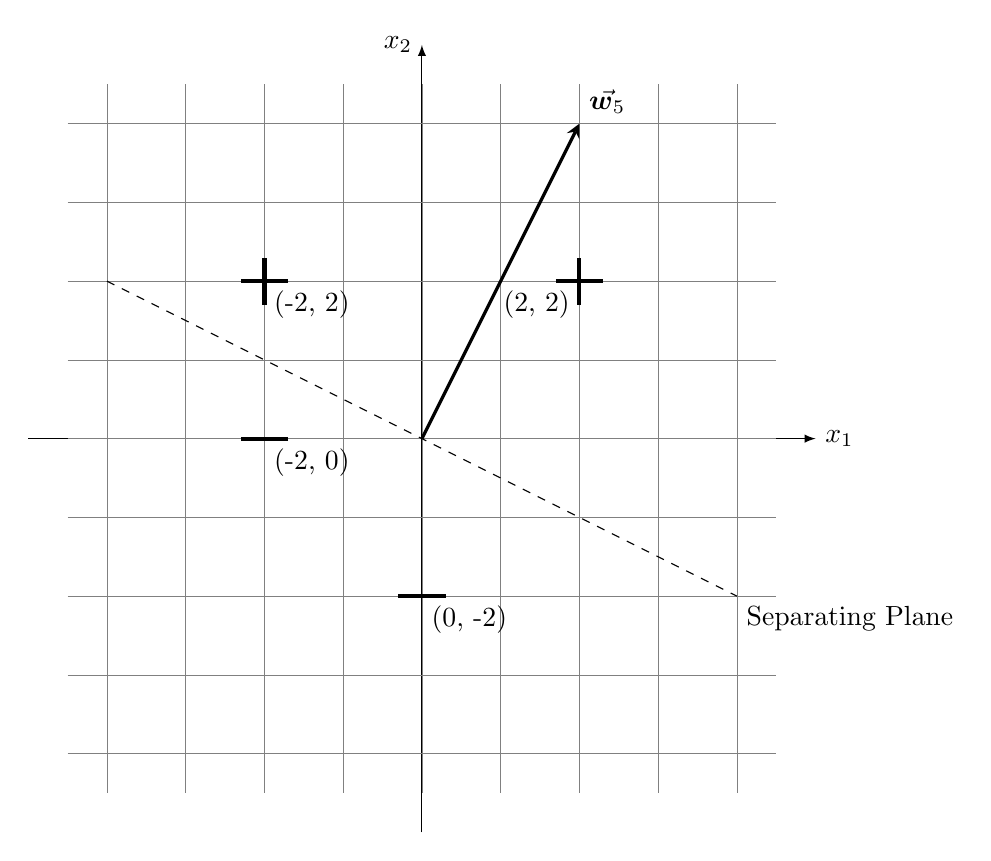
\begin{tikzpicture}
		\tikzstyle {point line} = [line width=0.15em]
								    
		\draw[-latex] (-5,0) -- (5,0) node[right]{$x_1$};
		\draw[-latex] (0,-5) -- (0,5) node[left]{$x_2$};
									
		\draw[help lines] (-4.5,-4.5) grid (4.5,4.5);
									
		\draw[point line] (-1.7,0) -- (-2.3,0);
		\draw[point line] (-0.3,-2) -- (0.3,-2);      
						
		\draw[point line] (-1.7,2) -- (-2.3,2);
		\draw[point line] (-2,1.7) -- (-2,2.3);  
						
		\draw[point line] (1.7,2) -- (2.3,2);
		\draw[point line] (2,1.7) -- (2,2.3); 	
						
		\draw (-2, 2) node [below right] {(-2, 2)};
		\draw (2, 2) node [below left] {(2, 2)};
		\draw (-2, 0) node [below right] {(-2, 0)};
		\draw (0, -2) node [below right] {(0, -2)};
											
		\draw [dashed] (-4, 2) -- (4, -2);
		\draw (4, -2) node [below right] {Separating Plane};   
										
		\draw[very thick,->, >=stealth] (0, 0) -- (2, 4);
		\draw (2, 4) node [above right] {$\vec{\boldsymbol{w}_5}$};  
						
	\end{tikzpicture}
\end{figure}

\FloatBarrier

\section{Proof of Convergence}

The intention is to show that the perceptron learning algorithm always converges to a perfect classifier in finite iterations given that all the assumptions that the algorithm makes are met.

 
Assume that after k+1 iterations, $\vec{\boldsymbol{w}_{k+1}}$ makes an angle $\theta_{k+1}$ with $\vec{\boldsymbol{w}^*}$. 
 
\begin{align*}
	cos(\theta_{k+1}) = \frac{\vec{\boldsymbol{w}_{k+1}}.\vec{\boldsymbol{w}^*}}{|\vec{\boldsymbol{w}_{k+1}}|\ |\vec{\boldsymbol{w}^*}|} 
\end{align*}
 
Since $\vec{\boldsymbol{w}^*}$ is a unit vector,
 
\begin{align*}
	cos(\theta_{k+1}) = \frac{\vec{\boldsymbol{w}_{k+1}}.\vec{\boldsymbol{w}^*}}{|\vec{\boldsymbol{w}_{k+1}}|} 
\end{align*}
 
Now, bounds for numerator and denominator are established to proceed ahead.
 
\subsection{Bound for numerator}
 
The update rule for $\vec{\boldsymbol{w}_{k+1}}$ is,
 
\begin{align*}
	\vec{\boldsymbol{w}_{k+1}} = \vec{\boldsymbol{w}_k} + y_i \vec{\boldsymbol{\boldsymbol{x}_i}} 
\end{align*}
 
Taking dot product with $\vec{\boldsymbol{w}^*}$ on both sides.
 
\begin{align*}
	\vec{\boldsymbol{w}^*}.\vec{\boldsymbol{w}_{k+1}} = \vec{\boldsymbol{w}^*}.\vec{\boldsymbol{w}_k} + y_i \vec{\boldsymbol{w}^*}.\vec{\boldsymbol{\boldsymbol{x}_i}} 
\end{align*} 
 
Since $y_i \vec{\boldsymbol{w}^*}.\vec{\boldsymbol{\boldsymbol{x}_i}} > \gamma$ as per the algorithm assumption.
 
\begin{align*}
	\vec{\boldsymbol{w}^*}.\vec{\boldsymbol{w}_{k+1}} > \vec{\boldsymbol{w}^*}.\vec{\boldsymbol{w}_k} + \gamma      \\
	\vec{\boldsymbol{w}^*}.\vec{\boldsymbol{w}_{k+1}} > \vec{\boldsymbol{w}^*}.\vec{\boldsymbol{w}_{k-1}} + 2\gamma \\
	\vec{\boldsymbol{w}^*}.\vec{\boldsymbol{w}_{k+1}} > \vec{\boldsymbol{w}^*}.\vec{\boldsymbol{w}_{1}} + k\gamma   
\end{align*}   
 
since $\vec{\boldsymbol{w}^*}.\vec{\boldsymbol{w}_{1}} = 0$.

 
\begin{align*}
	\vec{\boldsymbol{w}^*}.\vec{\boldsymbol{w}_{k+1}} >  k\gamma 
\end{align*}  
 
\subsection{Bound for denominator}
 
Again starting with the update rule for $\vec{\boldsymbol{w}_{k+1}}$,
 
\begin{align*}
	\vec{\boldsymbol{w}_{k+1}} = \vec{\boldsymbol{w}_k} + y_i \vec{\boldsymbol{\boldsymbol{x}_i}} 
\end{align*}
 
Taking modulus on both sides,
 
\begin{align*}
	|\vec{\boldsymbol{w}_{k+1}}|^2 = |\vec{\boldsymbol{w}_k}|^2 + |y_i \vec{\boldsymbol{\boldsymbol{x}_i}}|^2 + 2y_i \vec{\boldsymbol{w}_k}.\vec{\boldsymbol{\boldsymbol{x}_i}} 
\end{align*}
 
Since $y_i \vec{\boldsymbol{w}_k}.\vec{\boldsymbol{\boldsymbol{x}_i}} <= 0$ according to the algorithm specification.

\begin{align*}
	|\vec{\boldsymbol{w}_{k+1}}|^2 \leq |\vec{\boldsymbol{w}_k}|^2 + |y_i \vec{\boldsymbol{\boldsymbol{x}_i}}|^2 
\end{align*}
 
Assuming that the largest input vector has length $R$.
 
\begin{align*}
	|\vec{\boldsymbol{w}_{k+1}}|^2 \leq |\vec{\boldsymbol{w}_k}|^2 + R^2      \\
	|\vec{\boldsymbol{w}_{k+1}}|^2 \leq |\vec{\boldsymbol{w}_{k-1}}|^2 + 2R^2 \\
	|\vec{\boldsymbol{w}_{k+1}}|^2 \leq kR^2                                  \\
	|\vec{\boldsymbol{w}_{k+1}}| \leq \sqrt{k}R                               
\end{align*}
 
\subsection{Bound for Number of Iterations}
 
Using both the numerator and denominator bounds,

\begin{align*}
	cos(\theta_{k+1}) > \frac{k\gamma}{\sqrt{k}R} \\
	cos(\theta_{k+1}) > \sqrt{k} \frac{\gamma}{R} 
\end{align*}
 
This shows that after each iteration, the lower bound of the angle between $\vec{\boldsymbol{w}} $ and $\vec{\boldsymbol{w}^*}$ increases. And since $cos(\theta_{k+1})$ can never be greater than one, $\sqrt{k} \frac{\gamma}{R} \leq1$ must hold true yielding $k \leq \frac{R^2}{\gamma^2}$.

\section{Conclusion}

The perceptron was one of the first algorithms indicating that computers could learn from data. And today, after half a century, it continues to be the basis of Artificial Neural Networks which are at the forefront of Artificial Intelligence. 

\end{document}